\chapter{Experiments with DVI LCoS}
\begin{summary}
  Initially we strived to create a prototype, that would allow
  feedback between the spatial SLM and the camera with
  \unit[60]{Hz}. It was based on a fast ferroelectric liquid crystal
  on silicon device with DVI (digital video interface) data input as
  the spatial SLM.
  
  We overcame several problems with synchronization, latencies and
  light efficiency. Finally the remaining problems turned out to be
  too difficult to overcome\footnote{Retrospectively, there seems to
    be a solution which we mention in the discussion to this section.}
  and we rather switched to a spatial SLM solution with local storage
  as described in the main body in this work.

  Nevertheless we believe spatio-angular illumination with realtime
  control will be very useful and therefor we describe our system,
  even though it is impractical for now.
\end{summary}

\section{Description of the setup (fast MMA)}
The optical setup is the same as in \figref{fig:memi-real}. Sometimes
we use a blue LED diode array (CoolLed) instead of the laser as a
light source, that we couple with a fibre bundle into the integration
tunnel. The LED delivers less brightness but a more uniform
illumination -- especially of the MMA.

The ferroelectric LCoS display is nearly identical to the one used in
the main text (SXGA R3, ForthDD) but the data is transferred into the
controller from the computers graphics card via DVI. The computer
transmitts digital $24-$bit images ($1280\times1024$ pixels) with
$\unit[60]{Hz}$\footnote{Up to \unit[85]{Hz} are supported by the
  ferroelectric LCoS. This corresponds to a frame rate of
  $24\times\unit[85]{Hz}=\unit[2040]{Hz}$ of individual bit
  planes.}. The LCoS controller then displays a sequence of 24
bitplanes. Each bitplane is shown for $\unit[276.27]{\mu s}$ as
indicated in the \textsf{RED-ENABLE} signal in \figref{fig:trigger0}.

Originally the LCoS controller was designed by ForthDD to display
color images with 8 bits per color. In order to do this it would
display three times eight images of pulses, where each pulse would be
half the length of its predecessor. Three separate galvanically
decoupled TTL signals would then enable corresponding LEDs for red,
green and blue. We use the controller in a modified mode (48366
BitSlice 768-line 60Hz V1.0), where it would display each bitplane for
equal amounts of time and generate all light enable pulses on
\textsf{RED-ENABLE}.

Unfortunately the company doesn't provide the vertical sync signal
(which is generated by the graphics card in the computer). As a remedy
we use a microcontroller (Arduino) program (see code listing on page
\pageref{fig:arduino-vsync}), that reads the \textsf{RED-ENABLE} signal,
counts the pulses and measures the time between them. This way we are
able to find the longer gap of $\unit[587]{\mu s}$ infront of the
first pulse (which corresponds to bit 0 of the red byte).

% /home/martin/from-hp2-notebook/Downloads_pdf/Downloads4/Downloads/48366_BitSlice_768-line_60Hz.pdf

Initially we planned our device to run at the fastest possible
speed. The MMA has a delay of $\unit[850]{\mu s}$ between receiving a
trigger edge and the mirrors having settled in the requested
orientation. In order to run the MMA at a fast frame rate we decided
to generate a trigger pulse in the Arduino microcontroller after every
second LCoS bitplane\footnote{Note that microcontroller programming
  for synchronization requires a pecilular style. One must be careful
  about conditionals and loops. In order to have predictable pulse
  generation make sure each code path is run in the same time. It is
  best to unroll loops in order to prevent their initial
  overhead. Therefor we often generate these programs with another
  program.}. This gives enough time to the MMA controller to set the
mirrors and we can display simultaneous images on MMA and LCoS during
11 out of 24 LCoS bitplanes. The system therefor achieves a frame rate
of $\unit[60]{Hz}\times11=\unit[660]{Hz}$ and a duty cycle of just
$\unit[277]{\mu s}\times11\times\unit[60]{Hz}=0.18$.

\subsection{On using OGP1 as graphics hardware}
Using a graphics card to generate the images for the LCoS is a
non-optimal solution. A normal graphics card can't be externally
triggered. This means we can no longer have the slowest device (the
camera) as the master for synchronization and things will be either
slow or inflexible. Therefor we obtained a FPGA based graphics card
(the OGP1 from the open graphics project) which in principle could be
modified to generate the image, when requested. As it is still in
development stage its features were not fully developed. At the time
we were able to bring an image onto the LCoS but changing the content
of the video memory was rather slow (in the range of hundreds of
milliseconds) because it had to be done by direct access and drawing
operations or bitblt had not been implemented.

Later we learned from the manufacturer of the LCoS (ForthDD) that
varying the framerate at the DVI input would probably anyway not work.

\begin{figure}[!hbt]
  \centering
  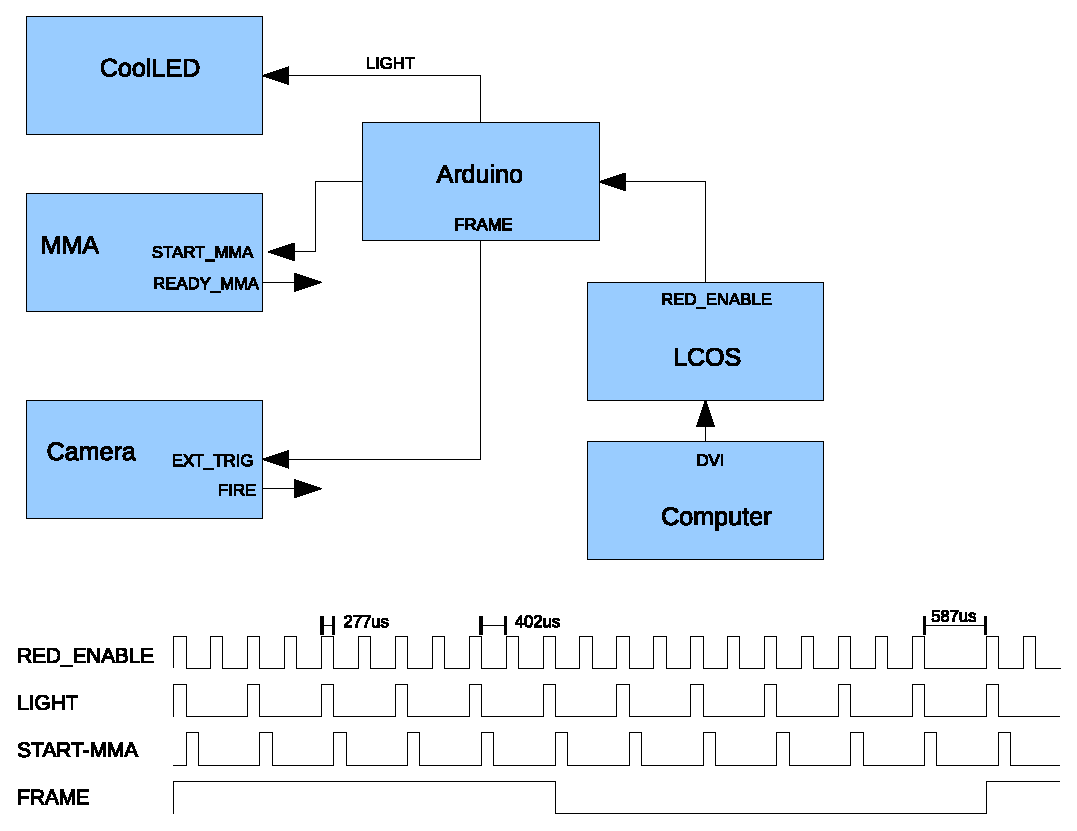
\includegraphics[width=12cm]{../dvi/trigger0}
  \caption{{\bf top:} Schematic of the electronic components of the
    system for the ``fast MMA'' trigger scheme. {\bf bottom:}
    Depiction of TTL trigger signals for this configuration. The
    \textsf{RED-ENABLE} signal is high, when the LCoS displays a
    bitplane. \textsf{LIGHT} enables the laser and \textsf{START-MMA}
    triggers the MMA, which displays an image after a delay of
    $\unit[850]{\mu s}$. The signal \textsf{FRAME} indicates the
    beginning of video frames and is necessary to start camera
    exposures at the right time.}
  \label{fig:trigger0}
\end{figure}


\section{Description of the trigger generation (slow MMA)}
We should note, that the MMA is a prototype as well and its
controller, though being connected to the computer via ethernet,
doesn't provide \unit[1]{Gbit/s} communication or any other means that
would allow realtime update of its image, e.g. support for run-length
encoding of the image data. Therefor the MMA can display images with
\unit[660]{Hz} but uploading one new image roughly takes
\unit[80]{ms}.

It therefor seems reasonable to switch to a different triggering
scheme, where the mirrors of the MMA are tilted for one full video
frame. The MMA has a limited maximum duty cycle of 50\%. This means we
have to drop every other frame from the graphics card. If camera
exposure times of \unit[16.66]{ms} are sufficient, we have even
doubled the duty cycle of the full system to $\unit[277]{\mu
  s}\times23\times\unit[60]{Hz}=0.38$. Note that we loose the first
bitplane due to the MMA's $\unit[850]{\mu s}$ load delay.

The z-stage of the microscope can perform $\unit[1]{\mu m}$ steps in
\unit[20]{ms}. Therefor displaying two black images on the LCoS (and
capturing one of them) is sufficient to ensure that the stage is at
the next position.

The following code listing shows the Arduino microcontroller programm,
that recovers the vsync signal from the pulse train on the
\textsf{RED-ENABLE} signal from the LCoS controller it generates pulses
with \unit[60]{Hz} on pin 13 that synchronize the MMA controller.
{\small\label{fig:arduino-vsync}
\begin{verbatim}
// takes the lcos signal (train of 24 pulses, followed by a pause)
// and generates a trigger signal for the mma at the end of each train
// so for every DVI image (consisting of 24 bit planes) a different
// mma image can be shown. 

volatile unsigned int Ticks;    // holds the pulse count as .5 us ticks
// pin 8 takes signal from lcos
char icpPin = 8;                // this interrupt handler must use pin 8
volatile char bit_plane_change = 0;  // incremented whenever a 
                                     // different bitplane is displayed
char mma = 13;                  // output towards mma

ISR (TIMER1_CAPT_vect) // interrupt gets called when pin 8 changes
{
        if (!bit_is_set (TCCR1B, ICES1)) // was rising edge detected?
                TCNT1 = 0;      // reset the counter
        else {                  // falling edge was detected
                Ticks = ICR1;
                if (Ticks > 1000) {
                        bit_plane_change = 0;
                }
        }
        TCCR1B ^= _BV (ICES1);  // toggle bit value to trigger on the
                                // other edge
        if (bit_plane_change == 47) {
                digitalWrite (mma, HIGH);
        }
        else if (bit_plane_change == 0) {
                digitalWrite (mma, LOW);
        }
        bit_plane_change++;
}
void setup ()                   // run once, when the sketch starts
{
        pinMode (icpPin, INPUT);
        pinMode (mma, OUTPUT);
        TCCR1A = 0x00;     // COM1A1=0, COM1A0=0 => Disconnect Pin OC1
                           //                     from Timer/Counter 1
                           // PWM11=0,PWM10=0 => PWM Operation disabled
        TCCR1B = 0x02;     // 16MHz clock with prescaler means TCNT1
                           // increments every .5 uS (cs11 bit set)
        Ticks = 0;         // default value indicating no pulse detected
        TIMSK1 = _BV (ICIE1); // enable input capture interrupt for timer 1
}
int getTick ()
{
        int akaTick;      // holds a copy of the tick count so we can
                          // return it after re-enabling interrupts
        cli ();           // disable interrupts
        akaTick = Ticks;
        sei ();           // enable interrupts
        return akaTick;
}
char get_plane_change ()
{
        int aka;
        cli ();
        aka = bit_plane_change;
        sei ();
        return aka;
}
void loop () {}                 
\end{verbatim}
}

Eventually, with generous support by a ForthDD engineer, we found a
way to access the vsync signal on the LCoS controller board, making
the above program obsolete. However, the process involved producing
our own circuit board because we needed to connect with an obscure SMD
size board to board connector and provide our own means of galvanic
isolation. Microcontroller programs, similar to the one above, have
since then proved quite useful to other members in our lab. 


\begin{figure}[!hbt]
  \centering
  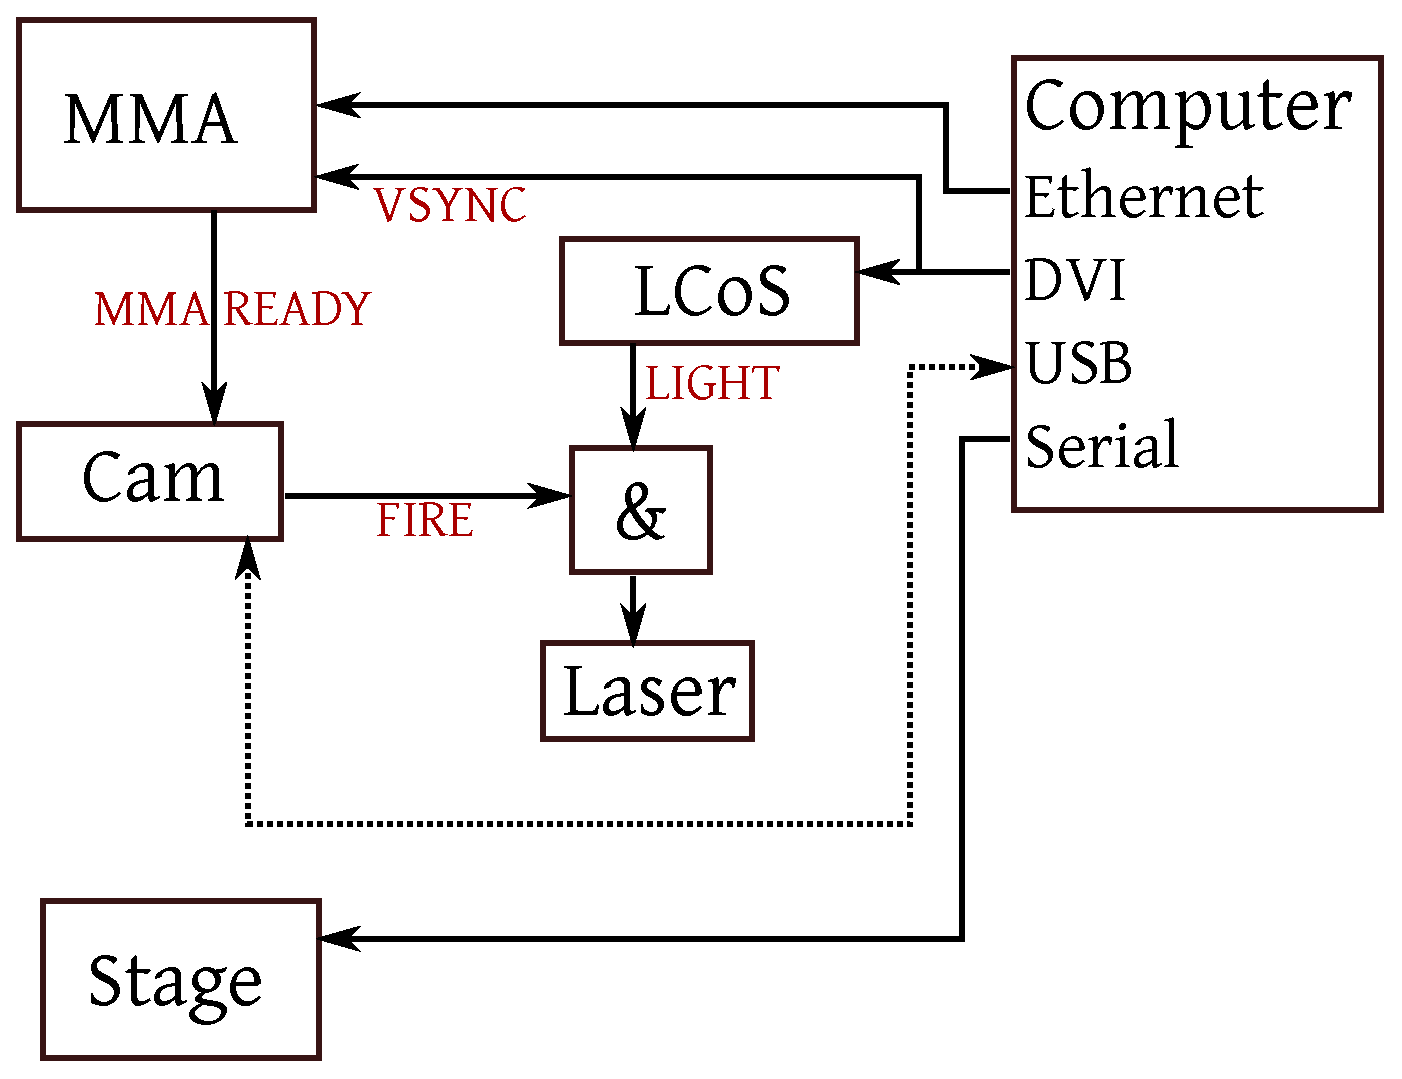
\includegraphics[width=8cm]{../dvi/09trigger}
  \caption{Schematic of the electronic system for the ``slow MMA''
    trigger scheme. The graphics card in the computer is the
    master. It generates images on the LCoS with \unit[60]{Hz}. The
    LCoS defines when the light can turn on but the Laser is only
    enabled, when the camera is integrating as well. The MMA selects
    only every second video frame from the graphics card and notifies
    the camera, when it has deflected its mirrors. The z-stage is controlled by the computer from within the display loop for the graphics card (synchronized with the signal \textsf{VSYNC}).  }
  \label{fig:09trigger}
\end{figure}



\begin{figure}[!hbt]
  \centering
  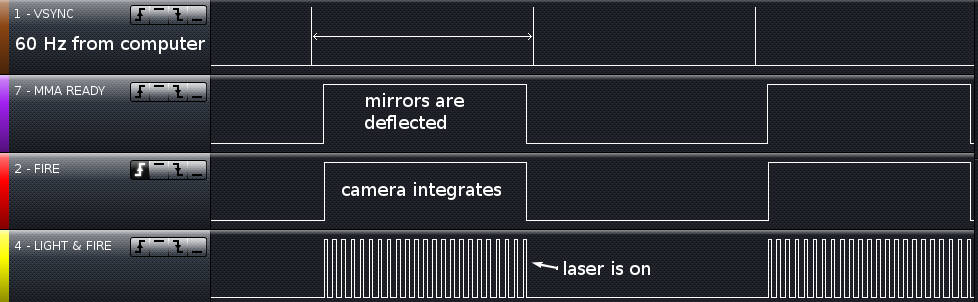
\includegraphics[width=12cm]{screen_logic_labels}
  \caption{Snapshot of the trigger signals for the ``slow MMA''
    configuration with a logic analyzer (Saleae Logic). The LCoS is
    the master, every second frame from the graphics card is
    integrated by the camera (which is running at \unit[30]{Hz}). The
    MMA has its mirrors tilted when the camera integrates, due to the
    delay of $\unit[850]{\mu s}$ the first image from the LCoS isn't
    collected in the exposure.}
  \label{fig:screen_logic_labels}
\end{figure}

\section{Verification of the synchronization}
In order to verify that the system is working, the graphics card is
displaying images with counters that incremented every frame (see
\figref{fig:fast4-no-first_cut}). As only every second image is
captured one would expect only odd counter numbers on the
camera. However, every 400 (or so) images a jump of on or more frames
occures. This problem can be traced back to the Steel Banks Common
Lisp\footnote{We used Common Lisp to develop most of our system. The
  main reason being an \unit[8]{s} initialization time in our camera's
  (Andor Clara) driver, that can't be disabled and hinders the C style
  edit--compile--run cycle.} garbage collector. A garbage collection
can take up to \unit[80]{ms}, which is not sufficient for the required
update rate of \unit[16]{ms}. Porting the code to C fixes this issue.

\begin{figure}[!hbt]
  \centering
  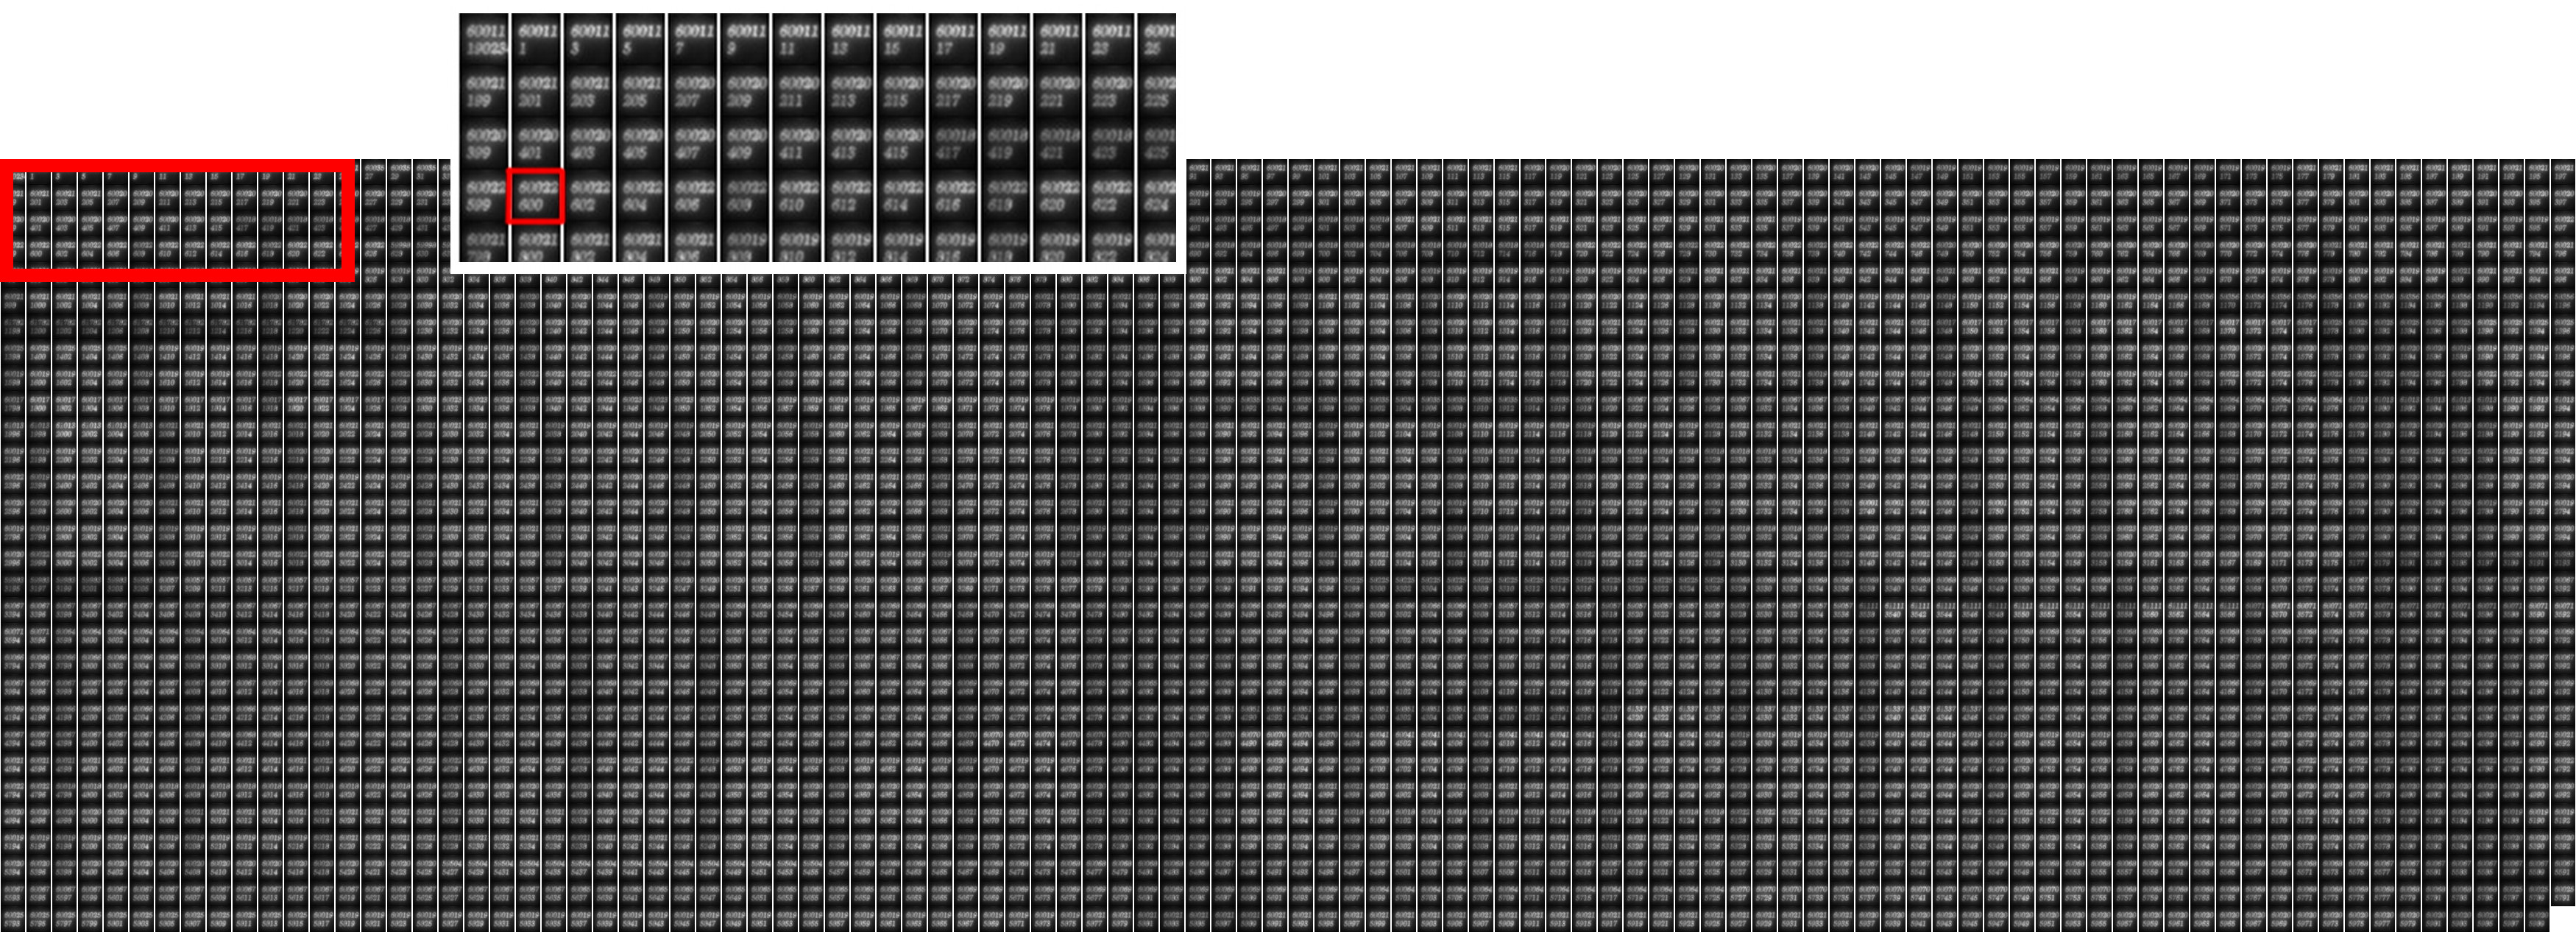
\includegraphics[width=14cm]{fast4-no-first_cut}
  \caption{Montage of many camera images captured in sequence. The
    LCoS was showing two frame counters. The bottom of the two numbers
    is reset at the beginning of the experiment and therefor counts
    $1,3,5,\ldots$. By design only every second image is
    captured. Occasionally a jump in the numbers was observed (see
    marked image) when the garbage collector ran. This was fixed by
    porting the code to C.}
  \label{fig:fast4-no-first_cut}
\end{figure}

The system was is now able to capture images with a rate of
\unit[30]{Hz} with a constant integration time of \unit[16]{ms}.  An
experiment has been devised, that can capture stacks of sectioned
data. In this acquisition protocol the MMA is not used for angular
control. It just displays white images and every fourth image a black
image. The LCoS displays three phases of a vertical grating and a
black image. When both displays show the black image, the stage moves
to the next slice. Capturing the slice and moving \unit[1]{$\mu m$}
takes eight video frames. A stack with 10 slices can be acquired in
\unit[1.3]{s}. \figref{fig:dvi-mosaic}~left shows images of a 3D
distribution of \unit[2]{$\mu m$} beads in agar acquired with this
imaging protocol.

The right mosaic in \figref{fig:dvi-mosaic} shows a reapplication of
the same acquisition protocol. However, there the devices didn't start
exactly at the same time. Maybe one in seven experiments, the
acquisition is successful. Trying to debug this problem proves
difficult.

On the one hand the camera doesn't provide time stamps, which would be
helpful to measure the latency between issuing the
\textsf{StartAcquistion} command and when the camera actually starts
integrating.  The same is true for the MMA. There is no specification
of how long \textsf{SLM-SetStartMMA} or
\textsf{SLM-SetPictureSequence} take and when the next incomming
trigger is processed.

One solution to the problem would be to display a sequence of patterns
in the beginning of each experiment that would allow the system to
recover the offset between the devices. An example pattern could be
five white images on the MMA ($+++++$), two dark double images on
LCoS, one dark LCoS double image, two dark LCoS double images ($--+--$).

By analyzing the camera images one could then recover when the bright
image arrived. The same procedure could be applied for the MMA as
well. In that case we would display $+++++$ on the LCoS and $--+--$ on
the MMA. This solution is rather cumbersome. Therefor we didn't try
it and replaced the LCoS with one that contains local storage.

\begin{figure}[!hbt]
  \centering
  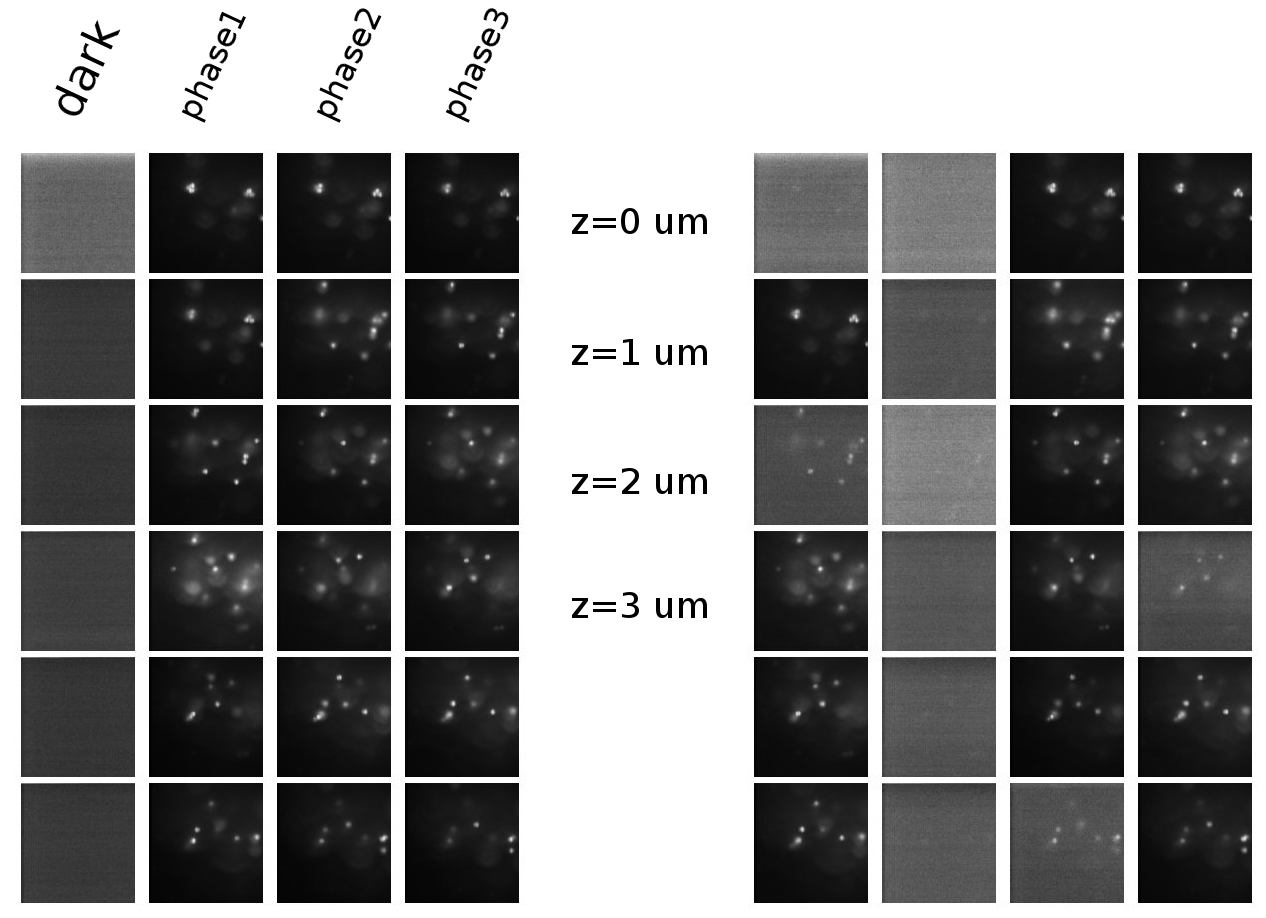
\includegraphics[width=10cm]{dvi-mosaic}
  \caption{{\bf left:} Sequence of images that was aquired while LCoS,
    MMA, z-stage and camera are running in sync. The camera is
    constantly running at \unit[30]{Hz} and the stage moves while a
    black mask is displayed on the MMA as well as the LCoS. The sample
    is a $\unit[2]{\mu m}$ yellow-green beads in agar {\bf right:}
    Same sequence of images should be displayed but the devices
    (camera, MMA and LCoS) do not start at the same time.}
  \label{fig:dvi-mosaic}
\end{figure}

\section{Conclusion}
The approach of sending data from the computer graphics card to the
LCoS by DVI would have its advantages but a synchronized start of
camera, MMA and LCoS proved to be too difficult or impractical.

If there was one display less, the approach would work perfectly fine.
Indeed we planned to build the optics using a spherical mirror and
bring conjugate planes of the pupil and the field (angular and spatial
control) next to each other on one LCoS.

We could have investigated the synchronization problem (e.g. camera
time stamps) further by sniffing data on the USB stack using the tool
Wireshark.

Another approach to solving the problem, is to generate a trigger
pulse from within the frame rendering loop in the computer
software. This pulse could ensure that all devices start running with
the same video frame.
